%
% OpenDCS Proposal
%
% Author: Geoff Johnson
%
% To compile: pdflatex --shell-escape --synctex=1 --interaction=nonstopmode proposal.tex
%

\documentclass[11pt]{article}

\usepackage[titles]{tocloft}
\usepackage{verbatim}
\usepackage[pdftex]{graphics,graphicx}
\usepackage[export]{adjustbox}
\usepackage{booktabs}
\usepackage{pdfpages}
\usepackage{float}
\usepackage{amssymb}
\usepackage{mathtools}
\usepackage{biblatex}
\usepackage{svg}
\usepackage{tikz}
\usepackage[tablegrid]{vhistory}
\usetikzlibrary{arrows}
\bibliography{references}

\usepackage{hyperref}
\hypersetup{%
  pdfauthor={Geoff Johnson},
  pdftitle={OpenDCS Project Proposal},
  pdfsubject={Project Proposal},
  pdfkeywords={OpenDCS Project Proposal},
  colorlinks=true,
  linkcolor=black,
  urlcolor=blue
}

% Packages used for appendices.
\usepackage{appendix}
\usepackage{listings}
\usepackage{color}
\definecolor{light-gray}{gray}{0.95}
\definecolor{listinggray}{gray}{0.9}
\definecolor{lbcolor}{rgb}{0.9,0.9,0.9}
\definecolor{light-blue}{rgb}{0.6,0.720,0.85}

% The default margins are too wide all the way around, reset them.
\setlength{\topmargin}{-.5in}
\setlength{\textheight}{9in}
\setlength{\oddsidemargin}{0in}
\setlength{\textwidth}{6.5in}

% Change paragraph formatting.
\setlength{\parindent}{0pt}
\setlength{\parskip}{2ex}

\begin{document}
\nocite{*}

  \title{%
    OpenDCS $-$ An Open Distributed Control System\vspace{2em}
  }

  \author{%
    Geoff Johnson \vspace{0.5em} \\
    geoff.jay@gmail.com \vspace{0.5em} \\
    A00533481 \vspace{0.5em} \\
    COMP8045 \vspace{0.5em}
  }

  \maketitle
  \thispagestyle{empty}
  \newpage
  \mbox{}
  \thispagestyle{empty}

  \newpage
  \addtocounter{page}{-1}
  \pagenumbering{roman}
  \tableofcontents
  %\listoffigures
  %\listoftables
  %\lstlistoflistings

  \newpage
  \pagenumbering{arabic}

  % XXX fill in or omit sections as needed, for now just blasting ideas

  % The institution of submission requires that this document contain
  % information about the student and company that the project is by/for.
  \section{Background}\label{sec:bg}

    \subsection{Student}\label{sec:bg-student}

      Geoff Johnson is a student of the BCIT Computer Systems Bachelor's degree.
      Prior to this he obtained a diploma of Computer Systems Technology from
      Camosun college in Victoria in 2001, as well as a diploma in Robotics and
      Automation Technology from BCIT in 2006.

      For the past 10 years Geoff has worked in Burnaby for the fluid mechanics
      research and development company Coanda where he is responsible for managing
      the IT operations, as well as managing and contributing to control system
      software development. This software is used to interface with industrial
      instrumentation, perform automated feedback control of plant processes,
      and capture data to log files at upwards of 100,000 samples per second.

    \subsection{Company}\label{sec:bg-company}

      Coanda is an engineering research and development company specializing in
      industrial fluid dynamics and related technologies. They have been in
      business for close to 20 years providing services in process flow modelling,
      design optimization, and custom instrumentation to name a few. For more
      information their website is \url{https://www.coanda.ca}.

    \subsection{Project}\label{sec:bg-project}

      The project being proposed is the reproduction of an existing piece of
      measurement and control software, implementing them as daemonized processes
      instead of the current all-in-one desktop application that is the current form.
      These server systems would be responsible for managing the process control,
      data logging, and data acquisition sub-processes. It should also implement a
      messaging API for setting and retrieving components of all data models,
      and a PUB/SUB socket system to allow these systems as well as other undefined
      clients to register to streamed data.

      While it may seem from this summary that the project lacks complexity the
      author would like to point out a couple of key reasons why this is an
      incorrect assumption. The existing software utilize a completely in-memory
      data model, there are no inter-process communication techniques utilized so
      moving to a completely different structure that utilizes a modern messaging
      platform is more than a simple rewrite and significant design and testing
      must be done to achieve accurate and reliable results. Additionally, while
      focussing on hardware access through the development of a device driver would
      be complex it would have little to no business value. Instead of focussing on
      recreating the wheel the design of this system will address how devices of
      any type can be easily integrated into a single cohesive system through the
      development of a module based architecture.

  \newpage

  % Describe the problem domain and issues at a high level.
  \section{Project Overview}\label{sec:desc}

    The current implementation is comprised of two software projects. The first is a
    library of objects that abstracts the data acquisition hardware as various
    types of measurement channels, it handles logging to both CSV files as well
    as databases, feedback control loop calculations using the PID (Proportional
    Integral Derivative) equation, and handles the creation of object hierarchy
    through a class builder using XML as the input. This library, libcld, is an
    open source project hosted as a git repository at
    \url{https://github.com/geoffjay/libcld}.

    The second piece of software, shown in Figure~\ref{fig:layout-dactl}, is an
    end user GUI application developed for the GNOME system. It interfaces with
    libcld, hereafter referred to as CLD (Control, Logging, and Data
    Acquisition), using a single context to provide the data necessary to
    update the interface view. This application has also been released as open
    source and is hosted at as a git repository at
    \url{https://github.com/coanda/dactl}.

    \begin{figure}[H]
      \centering
      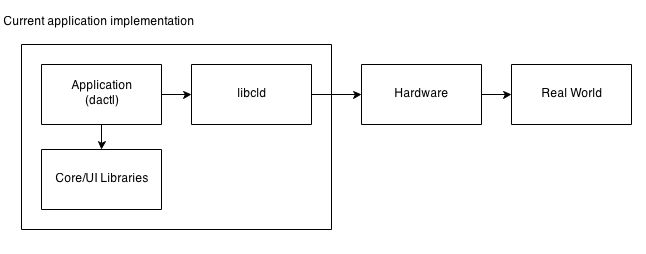
\includegraphics[scale=.6]{figures/dactl-current-layout.png}
      \caption{Current Application Design}\label{fig:layout-dactl}
    \end{figure}

    The proposed daemon solution is meant to address issues with the latter.
    Having high reliability tasks such as data acquisition and control reside in
    a GUI application that an unexperienced end-user operates can create reliability
    issues, sometimes through user mistakes, sometimes through issues with a
    graphical environment. A simple design of this proposed client/server
    platform is given in Figure~\ref{fig:layout-proposed-dcs}.

    \begin{figure}[H]
      \centering
      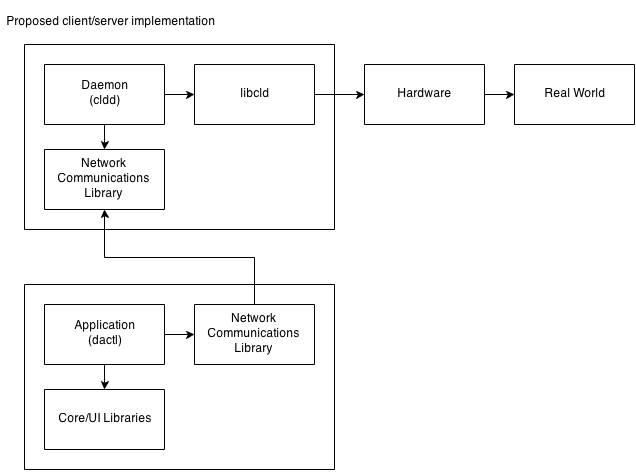
\includegraphics[scale=.5]{figures/dcs-proposed-layout.png}
      \caption{Proposed Client/Server Design}\label{fig:layout-proposed-dcs}
    \end{figure}

    %\subsection{Scope/Domain}\label{sec:desc-domain}

      %\subsubsection{Configuration Specification}\label{sec:desc-domain-conf}

      %\subsubsection{Instrument Measurement}\label{sec:desc-domain-instr}

      %\subsubsection{Automated Process Control}\label{sec:desc-domain-ctrl}

        %% FIXME: place the figure and equation side-by-side in a box
        %%\begin{figure}[htbp]
          %%\centering
          %%\includesvg[scale=.25,svgpath = figures/]{pid}
          %%\caption{PID Control Loop}
        %%\end{figure}

        %\begin{equation}
          %m_n = k_p*e_n + \frac{k_e*T}{T_{reset}}\sum_{i=0}^{n}e_i + k_d\frac{e_n - e_{n-1}}{\delta t} + m_{R}
        %\end{equation}

      %\subsubsection{Data Logging}\label{sec:desc-domain-logging}

      %\subsubsection{Plugin Framework Allowing for Device Type Expansion}\label{sec:desc-domain-plugin}

  \section{Technical Obstacles}\label{sec:tech-obstacles}

    Many of the technical obstacles presented by this project are likely going
    to be due to the desire to include unknown devices which communicate over
    different protocols and interfaces, for example RS232, I2C, TCP, SPI, etc.
    In order to address this problem directly the design and implementation of
    the underlying device library will be limited to an interface definition
    of a device modelled after a plugin, and a device loader.

    This architecture is already known to the developer and has been used in
    practice for a number of years. The device interface is a minimal
    description of what the derived plugins are capable of providing as well
    as defines what any must implement at a minimum to be understood by the
    system. For reference, this will use at an underlying level the well known
    and oft used libpeas which is included in the GNOME software ecosystem.

    The other source of potential technical hurdles is to do with both the
    messaging system chosen, ZeroMQ, and the implementation of a CRUD APIs
    as RESTful services. Fortunately the developer is already familiar with
    using ZeroMQ in practice as well as with all of the networking principles
    associated with such a platform. Also with respect to RESTful services,
    the author has developed such systems that are used in a production
    environment using both Javascript/NodeJS and Vala as the development
    platforms.

  % The proposed treatment to the problem described.
  \section{Proposed Solution}\label{sec:soln}

    Performing all of the work in a single application for data acquisition,
    feedback control, and data logging is open to a variety of issues. Doing so
    limits hardware scalability, places critical operations onto systems running
    desktop software, and ties high reliability functions like plant control in
    the same process as the front end that the end user operates. These are just
    to name a few of the more obvious problems.

    The system being proposed in this document is one that implements all of
    the hardware access and logging functionality into a daemon that runs as a
    process detached from the plant operator that interacts with the GUI
    application. This server software will use an existing library to interface
    with the data acquisition hardware as well as perform the control and
    logging tasks, this aspect of the software is a reimplimentation of work
    that already exists in an application that is currently in use.

    New functionality that is planned is the definition and minimal
    implementation of a REST API, a messaging system for streaming data, and a
    configuration definition to allow for the reconfiguration of the daemon. The
    REST API is meant to provide a means for clients to make simple requests of
    the system like read a single measurement value or change a property value
    of one of the internal objects. ZeroMQ is to be used to implement the
    messaging system, it has several high level features including publish and
    subscribe socket types that can be used for a streaming data system, a
    request/reply structure for a higher performance version of the REST API,
    and a structure for bridging communications to allow for the reconfiguration
    of the server as a proxy or slave node in a distributed system.

    % Discuss the benefit the end user gains from the proposed system that they
    % are currently missing.
    \subsection{Business Value}\label{sec:soln-val}

      With the current system that the client has in place there are a number
      of components or concepts that if added would be of significant value:

      \begin{enumerate}
        \item ability to separate the control process from the one that
              performs the data acquisition
        \item ability to separate the data logging process from the one that
              performs the data acquisition
        \item separation of the user interface component from the systems that
              perform the data acquisition, the data logging, and the process
              control
        \item ability to add new and modern backends for storing data once it
              has been sent to the data logging process
        \item acquire data from devices on separate computers over a messaging
              system (ZeroMQ) that is capable of high bandwidths, protocol
              buffers, improved security during transmission, and availability
              to almost any other language
      \end{enumerate}

      While this project may not be able to achieve all of these in the given
      time frame a major objective is to define the framework that would enable
      these. This would be achieved by replicating an existing plugin framework
      that exists in the user interface application that already exists.

      The business value of the existing plugin framework has been realized many
      times to date, it has been responsible for connecting dozens of different
      devices over a number of communication protocols all with their own
      custom interface components without ever needing to recompile the core
      application. This has allowed the client to deliver upgrades to copies of
      the software that has been installed in remote locations to customers
      without ever changing the original application. Given this experience it
      is believed that by further extending other parts of the system through a
      similarly designed component methodology the ability to connect to new
      and more complicated devices, systems, and protocols would be possible.

    \subsection{Opportunities for Inovation}\label{sec:soln-innov}

      With a project such as this there are many areas to innovate. There are
      opportunities to address access options to a variety of exotic and
      bleeding edge hardware, transmission security, performance, and timing
      as it relates to disparate systems.

      Obviously the time frame and scope of this project is not large enough to
      be inclusive of all of these areas, but a couple of key areas for
      evaluation will be listed here and based on feedback from the institution
      and the client prioritized as necessary. In all cases the author would
      like to provide a framework for future development at a minimum.

      \subsubsection{Securing Message Transmission}\label{sec:soln-innov-sec}

        A major failing of many control protocols, and distributed control
        systems in general, is the lack of security that they provide and the
        ability they offer to interroperate with other similar systems. This is
        one of the areas that this project would attempt to address through the
        inclusion of some encryption technology.

        Encryption is an increasingly important topic and with systems such as
        the one described here they are often left up to the end user to provide
        the security as needed. A prime example of this is the Modbus protocol,
        this common protocol that was originally developed using serial
        standards but later extended to use TCP networks exposes information
        about complex and critical control systems in a variety of industries.
        If the network administrator of such a network has not taken the
        appropriate steps to protect such traffic from would-be attackers almost
        anything can be taken over with little information.

        As a component of this project the author would like to investigate the
        options that are available to wrap traffic in standards like SSL, as
        well as add authentication mechanisms. The justification for encryption
        through SSL is fairly straightforward, but the authentication mechanism
        may hold more significance as it relates to common business objectives.
        A network based system that controls devices, for instance a pump,
        should not be controllable by more than one individual at a time, this
        is functionality that is lacking from may similar systems.

      \subsubsection{Performance}\label{sec:soln-innov-perf}

        Another area of concern for similar systems is performance, it is not
        uncommon when designing such a system to have major performance
        limitations on crucial data acquisition components in terms of timing.
        Data rates for transmition from one device to another is commonly
        defined in terms of single digit Hz, for many applications this is
        insufficient. There are two topics of interest that would add great
        value to this project, protocol buffers and the development of a wire
        protocol.

        \emph{Protocol Buffers} are similar to XML serialization but they are
        generally simpler to design, up to 10 times smaller, and up to 100 times
        faster. Utilizing this platform agnostic technology not only speeds up
        communication, it also opens it up to a variety of language alternatives
        for platform expansion.

        \emph{Wire Protocol} refers to a common method of representing data at
        the application level. Utilizing ZeroMQ's ability to be extended into
        custom wire protocols along with protocol buffers in a binary form has
        a large potential for a gain in overall performance of communication.

      \subsubsection{Precise Timing Protocol}\label{sec:soln-innov-ptp}

        Timing is a crucial component of data acquisition, not only the
        transmission time of a measurement, but also the accuracy and the
        ability for separate systems to be aware of when exactly some value
        was acquired. An example of this is where a system that is responsible
        for logging data receives from multiple others that acquire it, should
        the timing of the value logged be when it arrived at the logger, or
        when it was transmitted? The latter of the two makes the most sense
        except when you consider that those two systems may not have the same
        time.

        PTP is an existing protocol meant to address accuracy and
        synchronization issues in clocks throughout a computer network. On a
        LAN it is capable of achieving sub-microsecond accuracy which makes
        it suitable for a distributed control system.

        As part of this project it would be beneficial to research the
        inclusion of PTP, and to evaluate the accuracy and ability to reliably
        synchronize the multiple systems through a number of tests. This would
        require the inclusion of the protocol as well as defining how a system
        designer would be expected to structure the end system.

    \subsection{Development Process Model}\label{sec:soln-model}

      The current system that is in place and developed by the client is done
      so using what best fits the \emph{Rapid Application Development} process,
      this project will instead use an \emph{Incremental Development} process.
      Doing so leaves the project in a state at the end to either transition
      back to what the client prefers, or continue on using a more rigorous but
      still a reasonably fast paced methodology that can accomodate the needs
      of the business.

      Of significant concern for this project at the early phase is getting the
      requirements and design in a state that they can be used for more than a
      single iteration of the process, this is because the actual scope of such
      a system would be much more than would be possible in the time given.
      With that said, only a single full iteration is planned with extra
      emphasis during the analysis and design stages, this will hopefully
      reduce these in later iterations and allow for faster subsequent
      iterations.

      \subsubsection{Analysis}\label{sec:soln-model-analysis}

        During the analysis phase of the project all components will be
        identified by the client, fortunately many of these are already known
        so this is in part a review as well as a stage to catch additional unknown
        concerns. Once the project stakeholders have been identified and these
        have been defined the process of eliciting requirements will take place
        in the form of a series of meetings, the results of which will be
        recorded and used as input into the creation of SRS documents.

        After the process of gathering and analyzing the requirements has been
        completed they will be recorded using use cases or process
        specifications where applicable.

      \subsubsection{Design}\label{sec:soln-model-design}

        The software design process will be made up of two key components. The
        first is a series of \emph{Software Specification Design Documents}
        (SDD), and the second is a set of UML diagrams for the object-oriented
        libraries the are core to the system.

        The SDD for each component will describe at a minimum the criteria used
        for completion, and any milestones. For any applications where an
        interface is required, either graphical or otherwise, the SDD will
        include content regarding what the interface is meant to provide. It is
        unlikely that a graphical application will be a component of the design,
        but there is a high likelihood that the daemon processes will have a
        REST API that is the equivalent of the interface requiring a
        description.

        Given that components of this project are object-oriented, it is
        something that is sensible to include, if not required. UML is a method
        of describing components of a system visually by representing
        activities, components and their interactions, and any
        interfaces~\citation{WikiUML2016}. Ideally, these diagrams would feed
        into the Unit Test framework in a very significant manner.

      \subsubsection{Implementation}\label{sec:soln-model-implementation}

        The deployment target for this project is Linux and the various modern
        distributions that relate to it, as such the tools used for the
        implementation need to be ones that are consistent with it. This phase
        consists of not only the actual code that is compiled into the end
        result, but additional code projects that make up the build steps which
        use autotools for example, the documentation which will use the valadoc
        and possibly sphinx systems, and time permitting \emph{.deb}/\emph{.deb}
        packaging persuant to client desires regarding ease of deployment.

        Implementation will start with the build sections, where depending on
        the language and platform used can be either autotools/automake in the
        case where the code used is C or Vala, or a simple package system for
        bundling where the code used is Node Javascript or Ruby.

      \subsubsection{Testing}\label{sec:soln-model-testing}

        Software testing will be achieved for this project in two ways
        depending on the unit being tested. The subprojects that are developed
        as libraries will have written an unit test system with the goal to
        reach a percentage of code coverage that will be agreed upon with the
        client during the requirements stage, this document has assumed a value
        of 75$\%$ in Section~\ref{sec:eval}. Other subprojects that are
        developed as network daemons will rely on test clients and functional
        testing that will be developed to meet design specifications ultimately
        defined by the client during the design stage.

        The unit test framework that the author is familiar with is the
        Vala/GObject classes and assertions that are part of those softwares,
        an example of this can be seen in the
        \href{https://github.com/geoffjay/libcld/tree/master/tests}{libcld} git
        repository. This is object oriented when used with the Vala programming
        language and will therefore match well with the proposed development of
        the suite of libraries required to make this project successful.

        For the daemon application development it makes more sense to develop
        testing systems that are functional in nature as the actual functionality
        of the system is what needs to be tested. To achieve useful results the
        functional testing will be split into:

        \begin{itemize}
          \item \textbf{Network Design} - Validate from each system that every
                other networked system is visible and configured appropriately
                for communication. Unfortunately ZeroMQ can not be monitored
                using tcpdump or Wireshark at this time so custom test clients
                must be developed for evaluation.
          \item \textbf{Configuration} - Validate that the configuration of
                all daemon processes and the internal data models are coherent
                in terms of structure and their capacity for internal
                reference.
          \item \textbf{Configuration Validation} - Validate the configuration
                of all daemon processes in terms of syntax by creating schema
                definitions and having a test stage which applies it to the
                configuration provided.
          \item \textbf{Transmission Completion} - Validate the transmission
                as received by any subscribing system to the publishing system
                by creating several known messages which can be requested, for
                each a CRC will be calculated and known to both sides of the
                transmission.
        \end{itemize}

      \subsubsection{Deployment}\label{sec:soln-model-deploy}

        The project will be managed as a series of \emph{git} repositories hosted
        on \emph{github.org} using the name `OpenDCS' under an organization named
        `open-dcs', `opendcs' has unfortunately already been claimed. This
        organization and the repositories within will provide the documentation
        necessary to allow any user of the system to build from source all of the
        components. Wherever possible continuous integration will be used to
        verify the current build status of the projects, this status will be shown
        using badges in the README sections of each of the projects making it
        visible to the user what state the software is currently in.

        Realistically, reaching a stable 1.0 release of everything contained in
        this project prior to the completion date is not feasible. Part of a
        stable release would be the creation of distributable packages, eg.
        \emph{.deb/.rpm/.dmg/.msi}, for their corresponding operating systems.
        However, it may make sense at some point during development to be able
        to install the software using a package management utility in Linux and use
        an automated build system such as Copr or Launchpad to aide in the creation
        of \emph{.rpm} or \emph{.deb}. This would be an ideal deployment strategy,
        but will only be done if installation from source is for some reason deemed
        to be excessively complex.

        Another possibility for deployment would be use Docker, container software
        which is growing in popularity for simplifying in the SysOps and DevOps
        processes. Creation of a Dockerfile for each project component would not
        be a complicated addition and may happen organically during the development
        life-cycle because of what it offers towards automating testing and any
        changes in required infrastructure.

    % Existing technologies needed to realize a solution.
    %\subsection{Hardware Requirements}\label{sec:soln-tech-hw}

    %\subsection{Software Requirements}\label{sec:soln-tech-sw}

      %\subsubsection{ZeroMQ for Messaging}\label{sec:soln-tech-sw-msg}

        %% why use 0MQ ???
        %% - protocol buffers
        %% - leaves option for RDMA
        %% - simple PUB/SUB implementation
        %% - well documented ability to create wire protocols

      %\subsubsection{Configuration and Communication Through CLD}\label{sec:soln-tech-cld}

  \section{Documentation}\label{sec:doc}

    OpenDCS will be developed as open source software and can therefore
    utilize many existing tools that offer free use to OSS projects. The
    components of the various systems will be documented using the following
    scheme:

    \begin{itemize}
      \item All software components will be hosted in an online source code
            repository system that is capable of rendering Markdown files as
            HTML, each will include sections on `Installation', `Usage',
            `Contributing', and which `License' has been used.
      \item All libraries will be developed using the Vala programming language
            and will use standard valadoc markup in the source files, API
            documentation will be generated using the tool of the same name.
      \item Any systems employing a REST API will most likely interact with an
            underlying data model, all of the documentation for the CRUD used
            by these systems will be documented along with the tool in the
            corresponding online code repository using standard Markdown format
            viewable in any web browser.
      \item The project as a whole will have a single website to pull in all of
            the associated systems, this will provide an overview of the
            project and consolidate the installation sections of each project
            into a single distilled version.
    \end{itemize}

    Examples of the documentation systems referenced:

    \begin{itemize}
      \item \href{https://en.wikipedia.org/wiki/Markdown}{Markdown}
      \item \href{http://valadoc.org}{valadoc}
      \item \href{http://theforeman.org/api/1.11/index.html}{CRUD}
    \end{itemize}

  \newpage

  \section{Evaluation}\label{sec:eval}

    While an outline of the test plans and methodologies therein were discussed
    in Section~\ref{sec:sol-model-testing}, this one will focus on the metrics
    that will be used to determine whether or not the project as a whole meets
    the objectives that have been set.

    These are:

    \begin{enumerate}
      \item A device plugin using an Arduino type microcontroller must work as
            an acquisition device.
      \item The acquisition daemon must provide data at 100 kS/s on the message
            bus.
      \item The time taken for a single measurement from the point of
            measurement to the point received by a process control component
            must take under 100 ms.
      \item All data must be received asynchronously by the data logging
            subsystem with no values lost, this may require a CRC or a simple
            data received volume totalizer for evaluation.
      \item Inclusion of any new components created as a plugin must be
            loadable at runtime of the process performing the inclusion without
            the need to recompile that subsystem.
      \item A code coverage number of \%75 or higher as reported by either an
            online service such as \url{https://coveralls.io} or locally using
            the \emph{gcov} application available in GNU Linux distributions.
    \end{enumerate}

    Some of these objectives involve a proof-of-concept implementation to
    determine success, in these cases it will be necessary to create example
    applications that receive data over the network and provide reports that
    will be presented to the client. These reports will be defined during the
    analysis stage of the project, and subsequently agreed upon with the
    client.

    The other objectives listed above that do not fit the category of the run
    and report approach given above will require the development of key metrics
    during the analysis stage as defined by the client. Additionally, and
    wherever possible, some of these objectives that are able to use continuous
    integration systems such as Jenkins or TravisCI will do some to determine
    current stability of the compilation process and likely to report the code
    coverage as a percentage using the unit test framework as described in
    Section~\ref{sec:soln-model-testing}.

  \newpage

  % Step-by-step details of the work required to achieve the proposed goal.
  \section{Work Plan}\label{sec:plan}

    The major work units within the project work plan will be listed as version
    numbers to coincide with the release tracking that will take place in the
    project management software named `redmine'.

    Time available to work on the project is dependant on the author's
    availability above an average 40 hour work week, with this in mind an
    average daily allotment has been given in 2 hour blocks. Accounting for
    a regular 4 week vacation schedule and statutory holidays the maximum time
    available between the date of the submission of this proposal and the
    final report submission date given in Table~\ref{tab:timeline} 440 hours.
    The total number of hours proposed in Table~\ref{tab:milestones} is 450
    hours.

    \subsection{Timeline}\label{sec:plan-time}

      \begin{table}[H]
        \centering
        \begin{tabular}{l p{4cm} p{4cm}}
          \toprule
          Major Unit & Start Date & End Date \\ [0.5ex]
          \midrule
          0.0.1 & June 18 & July 23 \\
          0.0.2 & July 24 & August 17 \\
          0.0.3 & August 18 & September 3 \\
          0.1.0 & September 4 & September 4 \\
          0.1.1 & September 5 & September 29 \\
          0.1.2 & October 2 & November 6 \\
          0.1.3 & November 7 & January 2 \\
          0.1.4 & January 3 & January 29 \\
          0.1.5 & January 30 & February 12 \\
          0.1.6 & February 13 & March 6 \\
          0.1.7 & March 9 & March 26 \\
          0.1.8 & March 27 & April 17 \\
          0.1.9 & April 20 & June 14 \\
          0.2.0 & June 17 & June 17 \\
          \bottomrule
        \end{tabular}
        \caption{Project Timeline}\label{tab:timeline}
      \end{table}

    \subsection{Tasks \& Activities}\label{sec:plan-tasks}

      \begin{itemize}
        \item[0.0.1] Requirements analysis
          \begin{itemize}
            \item[\emph{(1 hr)}] Identify stakeholders
            \item[\emph{(2 hr)}] Hold meeting with stakeholders to gather requirements
            \item[\emph{(2 hr)}] Analyze requirements to identify conflicts and ensure consistency
            \item[\emph{(2 hr)}] Itemize requirements for review and delivery to client
            \item[\emph{(4 hr)}] Create SRS for core library
            \item[\emph{(4 hr)}] Create SRS for device plugin library
            \item[\emph{(8 hr)}] Create SRS and use case for data acquisition daemon
            \item[\emph{(8 hr)}] Create SRS for use case process control daemon
            \item[\emph{(8 hr)}] Create SRS for use case data logger daemon
            \item[\emph{(1 hr)}] Review requirements with client
          \end{itemize}
        \item[0.0.2] Design
          \begin{itemize}
            \item[\emph{(1 hr)}] Define the role of the data acquisition daemon
            \item[\emph{(1 hr)}] Define the role of the process control daemon
            \item[\emph{(1 hr)}] Define the role of the data logger daemon
            \item[\emph{(2 hr)}] Define configuration specification for data acquisition daemon
            \item[\emph{(2 hr)}] Define configuration specification for process control daemon
            \item[\emph{(2 hr)}] Define configuration specification for data logger daemon
            \item[\emph{(2 hr)}] Define REST API for data acquisition daemon
            \item[\emph{(2 hr)}] Define REST API for process control daemon
            \item[\emph{(2 hr)}] Define REST API for data logger daemon
            \item[\emph{(2 hr)}] Define specification for message publisher (data acquisition daemon)
            \item[\emph{(2 hr)}] Define failure conditions and expected responses for data acquisition daemon
            \item[\emph{(2 hr)}] Define failure conditions and expected responses for process control daemon
            \item[\emph{(2 hr)}] Define failure conditions and expected responses for data logger daemon
            \item[\emph{(4 hr)}] Consolidate preliminary design into an SDD for data acquisition daemon
            \item[\emph{(4 hr)}] Consolidate preliminary design into an SDD for process control daemon
            \item[\emph{(4 hr)}] Consolidate preliminary design into an SDD for data logger daemon
            \item[\emph{(1 hr)}] Review design with client
          \end{itemize}
        \item[0.0.3] System modeling
          \begin{itemize}
            \item[\emph{(8 hr)}] Create UML for core library
            \item[\emph{(8 hr)}] Create UML for device plugin library
            \item[\emph{(6 hr)}] Create UML for sample device plugin
            \item[\emph{(2 hr)}] Review design models with client
          \end{itemize}
        \item[0.1.0] Design approval
          \begin{itemize}
            \item[\emph{(1 hr)}] Initial review with subgroup of stakeholders
            \item[\emph{(1 hr)}] Edit design based on review
            \item[\emph{(2 hr)}] Meet with client to discuss final design and receive approval
          \end{itemize}
        \item[0.1.1] Code build systems
          \begin{itemize}
            \item[\emph{(8 hr)}] Write an autotools build system for the core library
            \item[\emph{(8 hr)}] Write an autotools build system for the device plugin library
            \item[\emph{(8 hr)}] Write an autotools build system for the data acquisition daemon
            \item[\emph{(8 hr)}] Write an autotools build system for the process control daemon
            \item[\emph{(4 hr)}] Create a NodeJS module project for the data logger daemon
            \item[\emph{(2 hr)}] Validate build and installation for the core library
            \item[\emph{(2 hr)}] Validate build and installation for the device plugin library
            \item[\emph{(2 hr)}] Validate build and installation for the data acquisition daemon
            \item[\emph{(2 hr)}] Validate build and installation for the process control daemon
            \item[\emph{(1 hr)}] Validate installation for the data logger daemon
          \end{itemize}
        \item[0.1.2] Core library development
          \begin{itemize}
            \item[\emph{(1 hr)}] Create project structure
            \item[\emph{(4 hr)}] Write class framework
            \item[\emph{(2 hr)}] Write class documentation using design documents
            \item[\emph{(2 hr)}] Write API documentation using desing documents
            \item[\emph{(4 hr)}] Create unit test framework
            \item[\emph{(16 hr)}] Code units tests
            \item[\emph{(16 hr)}] Code library
          \end{itemize}
        \item[0.1.3] Device plugin library development
          \begin{itemize}
            \item[\emph{(1 hr)}] Create project structure
            \item[\emph{(1 hr)}] Write class framework
            \item[\emph{(2 hr)}] Write class documentation using design documents
            \item[\emph{(2 hr)}] Write API documentation using desing documents
            \item[\emph{(4 hr)}] Create unit test framework
            \item[\emph{(16 hr)}] Code units tests
            \item[\emph{(16 hr)}] Code library
          \end{itemize}
        \item[0.1.4] Data acquisition daemon development
          \begin{itemize}
            \item[\emph{(2 hr)}] Create project structure
            \item[\emph{(8 hr)}] Write documentation using design documents
            \item[\emph{(4 hr)}] Write REST API CRUD documentation using design documents
            \item[\emph{(14 hr)}] Code prototype of daemon
            \item[\emph{(4 hr)}] Write simple example program as proof-of-concept
          \end{itemize}
        \item[0.1.5] Test device / plugin template creation
          \begin{itemize}
            \item[\emph{(8 hr)}] Write test device plugin template using C as the language
            \item[\emph{(8 hr)}] Write test device plugin template using Vala as the language
            \item[\emph{(4 hr)}] Write test device plugin template using Python as the language
            \item[\emph{(4 hr)}] Write test device plugin template using Javascript as the language
          \end{itemize}
        \item[0.1.6] Process control daemon development
          \begin{itemize}
            \item[\emph{(2 hr)}] Create project structure
            \item[\emph{(8 hr)}] Write documentation using design documents
            \item[\emph{(4 hr)}] Write REST API CRUD documentation using design documents
            \item[\emph{(12 hr)}] Code prototype of daemon
            \item[\emph{(4 hr)}] Write simple example program as proof-of-concept
          \end{itemize}
        \item[0.1.7] Data logger daemon development
          \begin{itemize}
            \item[\emph{(2 hr)}] Create project structure
            \item[\emph{(6 hr)}] Write documentation using design documents
            \item[\emph{(2 hr)}] Write REST API CRUD documentation using design documents
            \item[\emph{(12 hr)}] Code prototype of daemon
            \item[\emph{(4 hr)}] Write simple example program as proof-of-concept
          \end{itemize}
        \item[0.1.8] Example client development / Daemon benchmark tools
          \begin{itemize}
            \item[\emph{(8 hr)}] Write a data acquistion client for testing and benchmarking purposes
            \item[\emph{(6 hr)}] Write a process control client for testing and benchmarking purposes
            \item[\emph{(4 hr)}] Write a data logger client for testing and benchmarking purposes
            \item[\emph{(2 hr)}] Verify the data acquisition daemon using test/benchmark tool
            \item[\emph{(2 hr)}] Verify the process control daemon using test/benchmark tool
            \item[\emph{(2 hr)}] Verify the data logger daemon using test/benchmark tool
          \end{itemize}
        \item[0.1.9] Data analysis and report writing
          \begin{itemize}
            \item[\emph{(8 hr)}] Gather results from all unit test plans
            \item[\emph{(8 hr)}] Gather results from benchmark test clients/tools
            \item[\emph{(8 hr)}] Analyze results
            \item[\emph{(32 hr)}] Write final report
            \item[\emph{(2 hr)}] Review draft of final report to client
            \item[\emph{(16 hr)}] Perform edits
          \end{itemize}
        \item[0.2.0] Final report submission
          \begin{itemize}
            \item[\emph{(1 hr)}] Final document review
            \item[\emph{(2 hr)}] Meet with client to review report
            \item[\emph{(1 hr)}] Submit report to BCIT
          \end{itemize}
      \end{itemize}

    \subsection{Milestones}\label{sec:plan-milestones}

      \begin{table}[H]
        \centering
        \begin{tabular}{l p{12cm} l}
          \toprule
          Milestone & Description & Hours \\ [0.5ex]
          \midrule
          0.0.1 & Requirements analysis with complete SRS documents & 40 \\
          0.0.2 & Initial design and description with complete SDDs & 38 \\
          0.0.3 & UML design of software libraries complete & 24 \\
          0.1.0 & Design approved by client & 4 \\
          0.1.1 & Complete build framework with definition of all systems & 45 \\
          0.1.2 & Core library, unit test framework, and API documentation complete & 45 \\
          0.1.3 & DAQ device library, unit test framework, and API documentation complete & 42 \\
          0.1.4 & DAQ daemon framework, documentation, and REST API CRUD complete & 32 \\
          0.1.5 & Test device plugin skeleton and documentation created for C, Vala, Python, and Javascript & 24 \\
          0.1.6 & Process control daemon framework, documentation, and REST API CRUD complete & 30 \\
          0.1.7 & Data logger daemon framework, documentation, and REST API CRUD complete & 26 \\
          0.1.8 & Example clients written to evaluate acquisition, process control, and data logging daemons & 24 \\
          0.1.9 & Reports and results from testing consolidated and evaluated & 72 \\
          0.2.0 & Final report submitted & 4 \\
          \midrule
           & & 450 \\
          \bottomrule
        \end{tabular}
        \caption{Project Milestones}\label{tab:milestones}
      \end{table}

  % Insert a list of references that were cited.
  %\newpage
  %\printbibliography%

  % Appendices
  \newpage
  \addappheadtotoc%
  \appendix
  \appendixpage%

  % Left over from a previous proposal document, edit later as needed.
  \section{Glossary of Abbreviations and Terms}\label{app:glossary}

    Abbreviations and terms used within this document for computing and
    software related topics are given in Table~\ref{tab:gloss:sw}, and in
    Table~\ref{tab:gloss:hw} for hardware and data acquisition related topics.

    \begin{table}[H]
      \centering
      \begin{tabular}{l p{10cm}}
        \toprule
        Term & Definition/Explanation \\ [0.5ex]
        \midrule
        API & Application Programming interface \\
        Client & Refers to the software application that communications with a daemon \\
        Container & Operating system level virtualization similar to chroot jails \\
        CRC & Cyclic Redundancy Check, an error checking mechanism \\
        CRUD & Create, Read, Update, Delete \\
        Daemon & Common term used to refer to a server application in a Linux system \\
        DevOps & A practice emphasizing collaboration between developers and IT professionals \\
        Docker & Container software applications used for DevOps and SysOps \\
        GLib & Standard set of Linux system libraries for the GNOME window manager \\
        GNU & A collection of applications, libraries, and developer tools \\
        GNOME & Open source dekstop environment software used with Linux systems \\
        GObject & A C type library to gain object oriented style features \\
        GUI & Graphical User Interface \\
        OSS & Open Source Software \\
        Perl & A high level programming language good for rapid development \\
        REST & Representational State Transfer \\
        RS232 & Serial communication devices that has been ubiquitous for decades \\
        SDD & Software Specification Design Document \\
        SRS & Software Requirements Specification \\
        SysOps & System operator of a multi-user computing system \\
        UML & Unified Modeling Language \\
        Vala & An object oriented programming language that uses GObject types \\
        valadoc & A documentation standard and tool for creating API descriptions \\
        XML & Extensible markup language, common for use in messaging systems \\
        \bottomrule
      \end{tabular}
      \caption{Glossary of Software Terms}\label{tab:gloss:sw}
    \end{table}

    \begin{table}[H]
      \centering
      \begin{tabular}{l p{10cm}}
        \toprule
        Term & Definition/Explanation \\ [0.5ex]
        \midrule
        Comedi & Open source hardware drivers for Control and Measurement Devices \\
        Container & Operating system level virtualization similar to chroot jails \\
        Data Acquisition & The act of gathering data from a real world process \\
        DAQ & Acronym for Data Acquisition \\
        Plant & Term commonly used for industrial control systems \\
        Watchdog & Standard concept for monitoring a vital systems heartbeat \\
        \bottomrule
      \end{tabular}
      \caption{Glossary of Hardware Terms}\label{tab:gloss:hw}
    \end{table}

  \section{Websites Referenced}\label{app:websites}

    A list of websites that have been referenced in this document. These have
    been presented here instead of wherever the hyperlink has been made
    because in some cases very long URLs in printed documents can be less useful
    than an active link in a digital one.

    \begin{table}[H]
      \centering
      \begin{tabular}{l p{10cm}}
        \toprule
        Name & URL \\ [0.5ex]
        \midrule
        Coanda     & https://www.coanda.ca \\
        CRUD       & https://en.wikipedia.org/wiki/Create,\_read,\_update\_and\_delete \\
        dactl      & https://github.com/coanda/dactl \\
        libcld     & https://github.com/geoffjay/libcld \\
        Markdown   & https://en.wikipedia.org/wiki/Markdown \\
        Unit tests & https://github.com/geoffjay/libcld/tree/master/tests \\
        Valadoc    & http://valadoc.org \\
        \bottomrule
      \end{tabular}
      \caption{URL Reference List}\label{tab:websites}
    \end{table}

  \newpage

  \section{Document Change Log}\label{app:changelog}

		The table below serves to track the key revisions made to this document for
 		change control purposes.

		\begin{versionhistory}
      \vhEntry{0.1}{2016-04-13}{Geoff Johnson}{submit initial proposal (pages: all)}
      \vhEntry{0.2}{2016-05-11}{Geoff Johnson}{revise proposal based on committee feedback (pages: 1, 5, 6 \& 18)}
      %\vhEntry{}{}{}{}{}
      %\vhEntry{}{}{}{}{}
		\end{versionhistory}

\end{document}
